\documentclass{article}
\usepackage{tikz}
\usetikzlibrary{shapes, arrows, calc}

\begin{document}

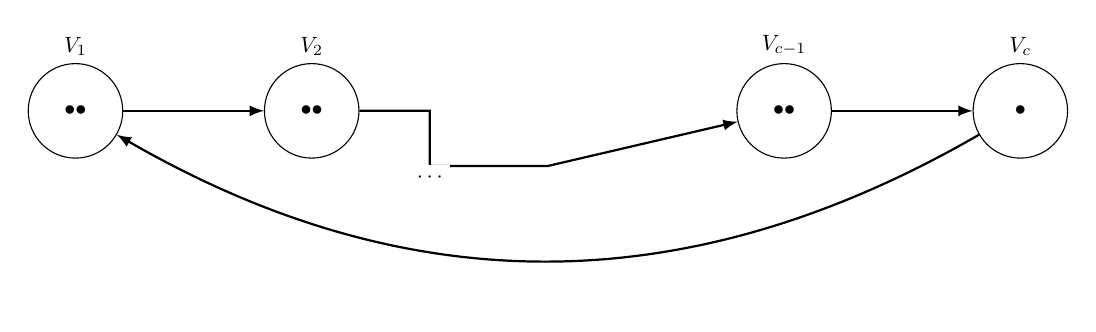
\begin{tikzpicture}[
    vertex/.style={circle, draw, minimum size=1.5cm, fill=white},
    arc/.style={-latex, thick},
    every node/.style={scale=0.8}
]

% Vertices
\node[vertex, label=above:$V_1$] (V1) at (0,0) {$\bullet$\\ $\bullet$};
\node[vertex, label=above:$V_2$] (V2) at (3,0) {$\bullet$\\ $\bullet$};
\node[vertex, label=above:$V_{c-1}$] (Vc-1) at (9,0) {$\bullet$\\ $\bullet$};
\node[vertex, label=above:$V_c$] (Vc) at (12,0) {$\bullet$};

% Arcs
\draw[arc] (V1) -- (V2);
\draw[arc] (V2) -- ++(1.5,0) -- ++(0,-0.7) -- ++(0,-0.3) node[midway, fill=white] {$\cdots$} -- ++(0,0.3) -- ++(1.5,0) -- (Vc-1);
\draw[arc] (Vc-1) -- (Vc);
\draw[arc] (Vc) to[out=-150,in=-30] (V1);

\end{tikzpicture}

\end{document}